\section{Koordinatni sistemi}
Orijentacija osa koordinatnog sistema preko kojih su određeni 
vektori ili tenzori potpuno je proizvoljna. Obično se jedna od osi(e.g. $x$ osa) poravnava 
sa geometrijskom osom tijela. 
Ako se tijelo kreće stalnom brzinom tada se jedan koordinatni sistem može 
koristiti za sve veličine, međutim ako se tijelo rotira tada se naslućuju dva koordinatna sistema:
\begin{itemize}
    \item Koordinatni sistem vezan za zemlju
    \item Koordinatni sistem vezan za tijelo
\end{itemize}
Koordinatni sistem vezan za zemlju je inertcijalni iako se zemlje rotira u odnosu na geomtrijsku osu.
Sastoji se od tri ordinate, jedna predstavlja poziciju po sjevernoj osi, jedna po lokaloj istočnoj osi 
i jedna predstavlja vertikalnu poziciju. Ose koordinatnog sistema vezanog za zemlju su 
označene sa $X_e, Y_e, Z_e$. Drugim riječima, $X_e$ i $Y_e$ leže u ravni dok je $Z_e$ usmjeren ka centru Zemlje.\\
Koordinatni sistem vezan za tijelo sastoji se iz tri ordinate sa ishodištem u centru gravitacije letjelice: $x$ osa koja je
usmjerena ka nosu letjelice tj. podudara se sa longitudinalnom osom, $y$ ose koja je usmjerena ka desnom krilu letjelice i $z$ ose koja dopunjava lijevo orijentisani 
koordinatni sistem.
\begin{figure}[h!]
    \centering
    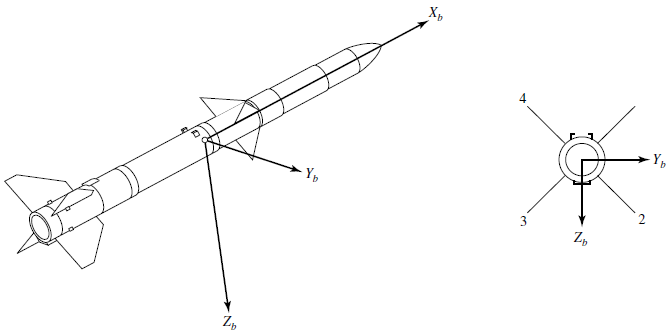
\includegraphics[scale=0.7]{body.png}
    \caption{Koordinatni sistem vezan za tijelo}
    \label{fig:KBS}
\end{figure}
Da se definiše položaj letjelice u odnosu na koordinatni sistem koriste se Eulerovi uglovi($\psi, \theta, \phi$).
\begin{figure}[h!]
    \centering
    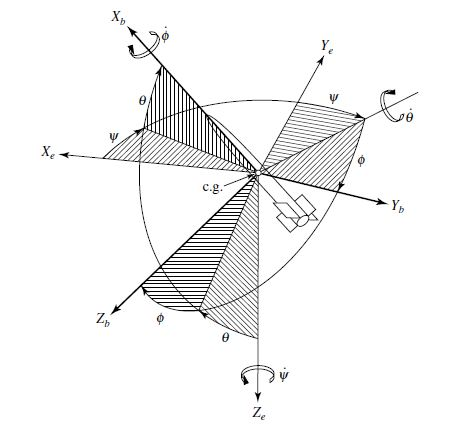
\includegraphics[scale=0.7]{earth-body.JPG}
    \caption{Eulerovi uglovi}
\end{figure}
Ovo znači da se bilo koja rotacija može postići sa tri rotacije oko osi i to prva 
rotacija za ugao $\phi$ oko longitudinalne, za ugao $\theta$ oko lateralne i za ugao 
$\psi$ oko normalne ose. Transformacija $C_e^b$ koja ostvaruje transformaciju iz 
koordinatnog sistema vezanog za zemlju u koordinatni sistem vezan za tijelo je data sa:
\begin{equation}    
    C_e^b=\begin{bmatrix}
        1&0&0\\
        0&\cos\phi & \sin\phi \\
        0 & -\sin\phi & \cos\phi \\
    \end{bmatrix}    
    \begin{bmatrix}
        \cos\theta&-\sin\theta&\\
        0&1 & 0 \\
        \sin\theta & 0 & \cos\theta \\
    \end{bmatrix}
    \begin{bmatrix}
        \cos\psi & \sin\psi & 0\\
        -\sin\psi & \cos\psi &0\\
        0&0&1\\
    \end{bmatrix}
\end{equation}
Treba primjetiti da rezultantna matrica $C_e^b$ može imati singularitete, pa se domen
Euloerovih uglova ograničava na sljedeći način:
\begin{align*}
    -\pi \leq \phi <\pi \quad ili \quad 0\leq\phi<2\pi \\
    -\pi \leq \psi <\pi \qquad \qquad \qquad \qquad \\
    -\frac{\pi}{2}\leq \theta \leq \frac{\pi}{2} \quad ili \quad 0\leq\psi<2\pi
\end{align*}
Ovo znači da u ovom slučaju postoji beskonačno mnogo načina da se ostvari željena transformacija.
Ovaj problem se može riješiti uvođenjem jediničnog kvaterniona.

\section{Jednačine kretanja čvrstog tijela}
Sada ćemo posmatrati tipični projektil i izvesti jednačine koje opisuju njegovo kretnaje.
Pretpostaviti će se da čvrsto tijelo nema promjena u obliku pri kretanju. Translacija tijela 
podrazumijeva da svaka duž koja spaja bilo koje dvije tačke u tijelu bude paralelna svojoj
datoj originalnoj poziciji, prema tome čvrsto tijelo se može posmatrati kao čestica čija je 
masa skoncentrisana u jednoj tački koja se zove \textit{centar mase}. Dalje se pretpostavlja 
da se oblik tijela ne mjenja usljed djelovanja sila na tijelo. Ovom pretpostavkom se 
dobija da međusobni utjecaj dijelića tijela eleiminisan pa se transalcija može potpuno opisati
translacijom centra mase i da se rotacija može potpuno opisati rotacijom oko centra mase. Dodatno 
pretpostavlja se da se ravan simetrije poklapa sa ravninom $X_b - Z_b$ kao što je to prikazano na 
slici \ref{fig:KBS}. Također pretpostavlja se da je masa tijela konstantna. Važno je 
napomenuti da se jednačine tijela određuju u koordinatnom sistemu vezanom za tijelo. 
Nadalje, projektil ima šest stepeni slobode(6-DOF). Ovih šest stepeni se sastoje iz od tri translacije i 
tri rotacije. Translacije se sastoje od kretanja duž osi $X_b,Y_b,Z_b$ brzinom $v_m=(u,v,w)$, a rotacije se sastoje 
od rotacija oko ovih osi ugaonom brzinom $\omega = (P,Q,R)$. Šest stepeni slobode je prikazano
na slici \ref{fig:dof} 
\begin{figure}
    \centering
    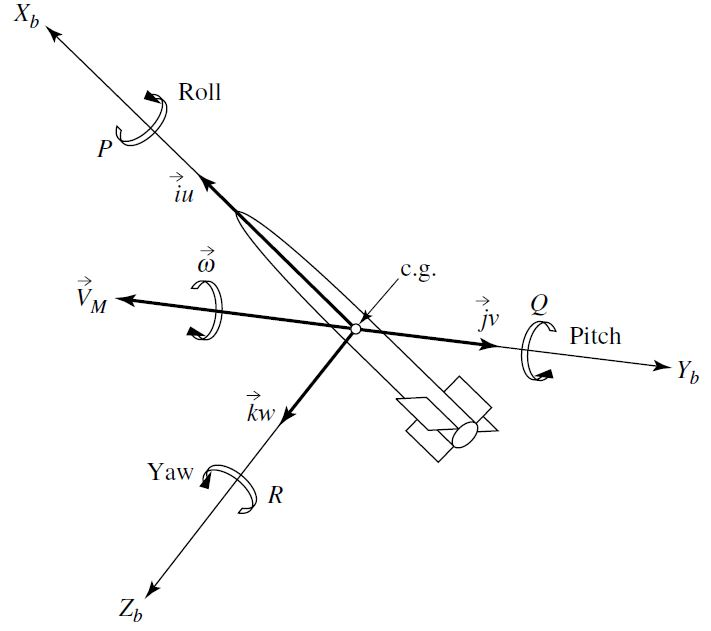
\includegraphics[scale=0.6]{6dof.JPG}
    \caption{Predstava šest stepeni slobode}
    \label{fig:dof}
\end{figure}